\section{Introduction}

\subsection{School}
\begin{figure}[ht]
    \centering
    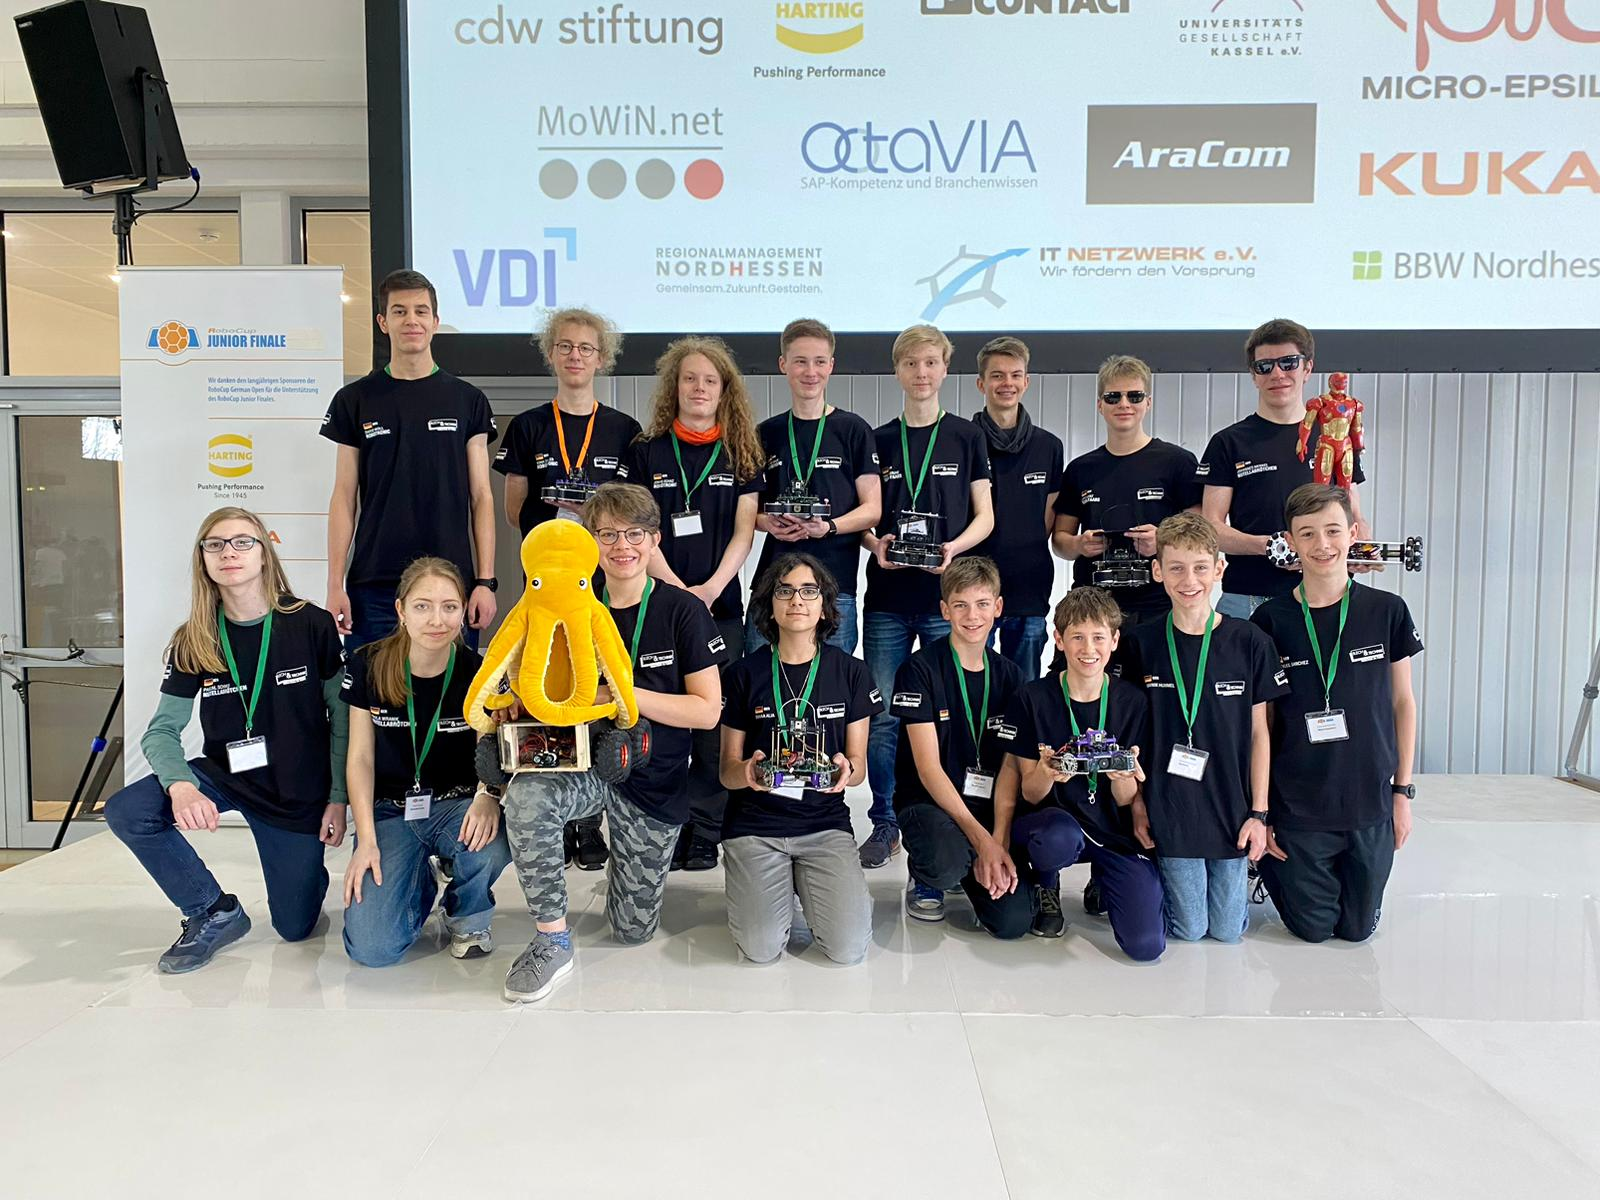
\includegraphics[width=\textwidth]{img/LGNU.jpg}
    \caption{Lessing Gymnasium Neu-Ulm - German Open}
    \label{fig:LGNU}
\end{figure}

\makeatletter
\providecommand{\rowno}[1][__empty__]{%
\ifthenelse{\isundefined{\c@rowno}}{%
\newcounter{rowno}}{}%
\ifthenelse{\equal{#1}{__empty__}}{%
\stepcounter{rowno}%
}{%
\setcounter{rowno}{#1}%
}%
\therowno.%
}
\makeatother

The Robotics program of our school was created 2011. Since then, we managed to win the World Open
multiple times in either Soccer LightWeight, Soccer Open or OnStage.
We try to put our new Teams as fast as possible in top leagues. With the gathered experience, we always
have teams to follow our footsteps.
\newpage

\subsection{Team}
\begin{figure}[h]
    \centering
    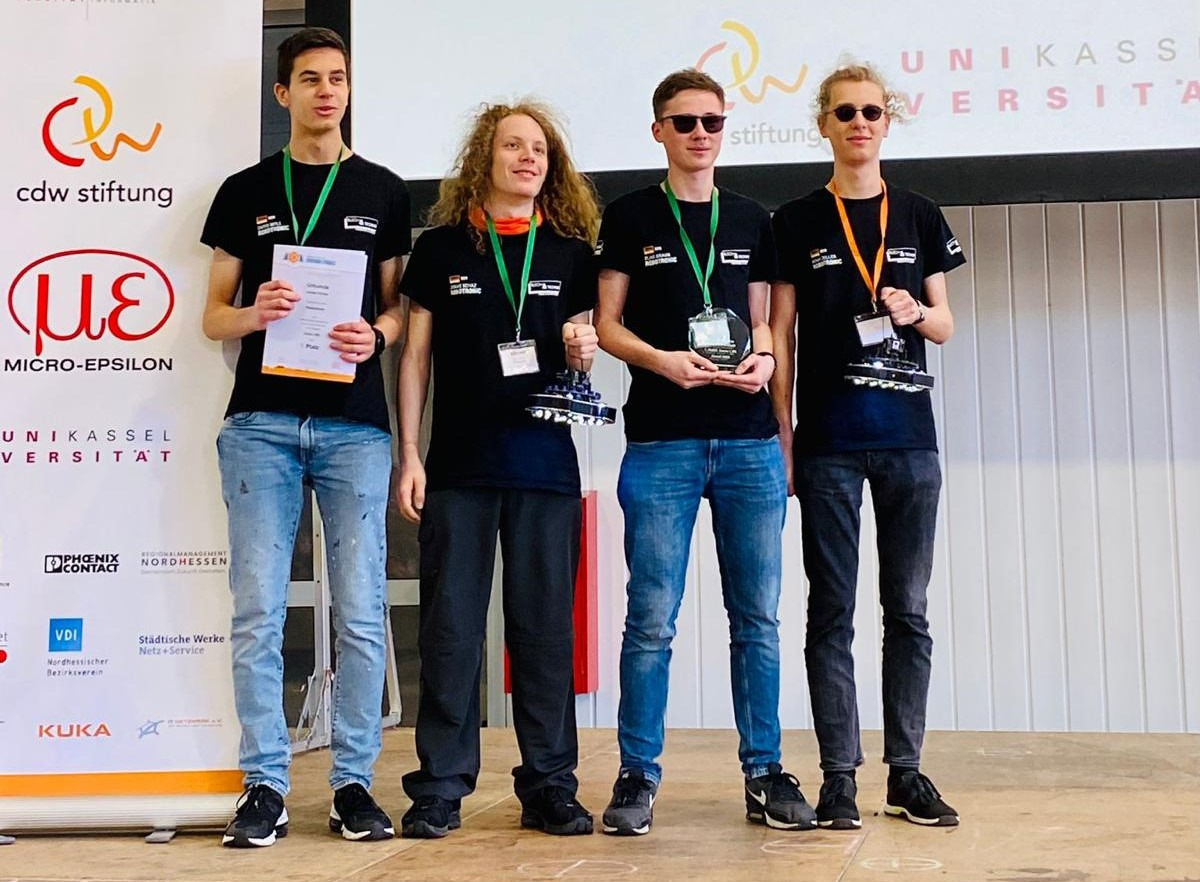
\includegraphics[width=\textwidth]{img/Robotronic.jpg}
    \caption{Team Robotronic - Dario Woll, Jonas Schaz, Elias Braun, Noah Zeller}
    \label{fig:team}
\end{figure}
In our Team, everyone has a specific task to do.\\


% \begin{enumerate}
%     \item{Dario Woll: Software $\rightarrow$ Calibration \& StepUp Design}
%     \item{Jonas Schaz: Software  $\rightarrow$ Ball Tracking, Mouse Sensor}
%     \item{Elias Braun: Hardware $\rightarrow$ Robot}
%     \item{Noah Zeller: Software $\rightarrow$ Compass, Camera}
% \end{enumerate}
\begin{tabular}[h]{r|c|l}
    Dario Woll&Software&Calibration \& StepUp Design\\\hline
    Jonas Schaz&Software&Ball Tracking \& Mouse Sensor\\\hline
    Elias Braun&Hardware&Robot\\\hline
    Noah Zeller&Software&Compass \& Camera
\end{tabular}
\newpage

\subsection{Abstract}
We are a Team of four students from the Lessing Gymnasium Neu-Ulm in Germany. Furthermore, we founded our Team
in 2018 and first participated in the RoboCup Junior in 2019. Robotic is a big part of our daily life.
We meet on school days and even on weekends and Holidays.
\newline
\newline
We started developing our Robots in mid 2022 and had a first Prototype in late 2022. After final design
choices, we had our Robots for the South-Open in early 2023. From this point on, not much progress was
made in the Hardware sector.
After a lot of programming, we managed to reach the second place.
\newline
After the South-Open we redesigned the Top Part of the Robot. We discovered, that with two cameras
instead of one we would have more opportunities in software instead of one camera and ultrasonic sensors.
With these improvements we managed to win the German Open.